\documentclass[11pt]{amsart}
\usepackage{geometry}
\geometry{letterpaper}
\usepackage{graphicx}
\usepackage{amssymb}
\usepackage{amsmath}
\usepackage{epstopdf}
\usepackage{fancyhdr}
\usepackage{tikz}
\usepackage{caption}


\def\DrawAirfoil#1{
  % NACA 2412
  \draw plot [smooth, scale=#1] coordinates {
    (1.0, -0.0012599999999999777)
    (0.96549018468297, -0.003766550717226144)
    (0.930883045462546, -0.006219202442366447)
    (0.8961437971575432, -0.008631733865730334)
    (0.8613016381510661, -0.011011201185171479)
    (0.8263867428041894, -0.013362379670991803)
    (0.7914310164102236, -0.015687541221114883)
    (0.7564670891854666, -0.01798637927354734)
    (0.7215286223342008, -0.020255875905877893)
    (0.6866502816986508, -0.022490225407487845)
    (0.6518674215422855, -0.02468081055332231)
    (0.6172164265648663, -0.026816170723141183)
    (0.5827346534458342, -0.02888202916719134)
    (0.5484605052100948, -0.03086134225579657)
    (0.5144339818074576, -0.032734349703361115)
    (0.480696823454966, -0.03447867568513195)
    (0.4472934967551756, -0.03606940997738771)
    (0.41393567802086406, -0.037492644839771605)
    (0.3804149998506693, -0.03874755535699173)
    (0.3468272731008735, -0.039902691513794025)
    (0.3136190982592265, -0.04090782505712402)
    (0.2811814440525585, -0.04170125833576889)
    (0.2496338451339312, -0.04222939050878645)
    (0.21912534718162296, -0.04243729854617861)
    (0.1898439100344943, -0.042270895665989155)
    (0.16202614783530983, -0.0416809040510345)
    (0.13596390146008333, -0.04062966635981699)
    (0.11199933361948029, -0.039101582938232377)
    (0.09049621574701124, -0.037116349985295505)
    (0.07361924489626276, -0.0350073364191772)
    (0.05636259357037546, -0.0321514577872086)
    (0.04397649402900053, -0.02948274558741349)
    (0.031214918278790867, -0.025913353166771468)
    (0.025386870661493165, -0.02387293613730815)
    (0.01986852747692683, -0.021588341403196154)
    (0.015810475611440528, -0.019602135923702295)
    (0.012032895834446736, -0.01741586159249026)
    (0.008347783658642402, -0.014804213953756641)
    (0.006782776357419023, -0.013476228004680135)
    (0.005101987955964444, -0.01182609576308366)
    (0.004152048570182651, -0.010748129365261013)
    (0.0030603428943254468, -0.009316573595328595)
    (0.0023446574801605675, -0.008213642891790378)
    (0.001731083959066247, -0.007107510715816521)
    (0.0012037942711423102, -0.005969188316183293)
    (0.0006943488170150654, -0.00457210891942128)
    (0.0002949883265427625, -0.0030077870143021875)
    (0.00013268271827913483, -0.002028658161884189)
    (0.000047353525254730774, -0.0012175353029981746)
    (0.00002532476506966959, 0.0008970844059684918)
    (0.00018814793077252665, 0.002448072322554881)
    (0.00037457810981088356, 0.00345681778994653)
    (0.0006226843506845091, 0.004460305424217867)
    (0.0009189939842633151, 0.0054224385524775705)
    (0.0016420541089524005, 0.007257797625008717)
    (0.0028235547140623278, 0.00953206869809826)
    (0.0039902533393324745, 0.01134485186269217)
    (0.00508347301295101, 0.012816488263046943)
    (0.006234932100785785, 0.014205330332066607)
    (0.008164412430203494, 0.016273130533696094)
    (0.0109096354233833, 0.01883301025054221)
    (0.0149335517829051, 0.022059247763182688)
    (0.02090169719548933, 0.026119219613711435)
    (0.029090969152910873, 0.0308133496989451)
    (0.03936014651201021, 0.03579205910007571)
    (0.05135871826960699, 0.040760579490798525)
    (0.06527912321719298, 0.04572188569496259)
    (0.08128812301403121, 0.05064207626527274)
    (0.09937610494377608, 0.05542524513564439)
    (0.11929438296032827, 0.0599347534152128)
    (0.14075992658866143, 0.06406441454515942)
    (0.1635174601103429, 0.06774419165547137)
    (0.18735476998529443, 0.07093243648306191)
    (0.21210090281011207, 0.07360721154371101)
    (0.23761935376120738, 0.0757595916459023)
    (0.2638006186070965, 0.07738903218729433)
    (0.29055586446557025, 0.07850032882407872)
    (0.31781188174707375, 0.07910164537520417)
    (0.34550708677686826, 0.07920323908566278)
    (0.37365456652101114, 0.07881517686907744)
    (0.402631894340016, 0.07793063620654582)
    (0.43241230840392214, 0.07660997118115524)
    (0.46290547434324336, 0.07490494347854927)
    (0.4936649080396488, 0.07284825058170255)
    (0.5246548772457837, 0.0704561000377626)
    (0.5558421106966199, 0.06774368002361203)
    (0.5871951553016743, 0.06472507690681442)
    (0.6186840935139319, 0.061413195624036104)
    (0.650280234781535, 0.05781970701641605)
    (0.6819560363938716, 0.053954993285283706)
    (0.7136849190124785, 0.049828124742128076)
    (0.7454411587455343, 0.045446849321571406)
    (0.7771999395698983, 0.040817578741059804)
    (0.8089371985433962, 0.0359454208624503)
    (0.840629806069205, 0.030834179949050796)
    (0.8722552320885923, 0.025486452979646447)
    (0.903791999768359, 0.01990361393618675)
    (0.935219453987816, 0.014085919535834577)
    (0.9672766290279255, 0.007882534061003747)
    (1.0, 0.0012599999999999777)
  };
}


\begin{document}

\begin{description}
  \item[Problem 1] A wing of span $b$ has a distributed lift force
    $l(x)$ along the top and is held down by bridles located at $b/4$
    and $3b/4$.  The bridles may be modeled as point loads going
    straight down with magnitude $T$ N each.  The distributed lift
    force is constant along the span with magnitude $2T/b$ N/m.  What
    are the shear and moment distributions along the wing?

    \begin{figure}[h]
      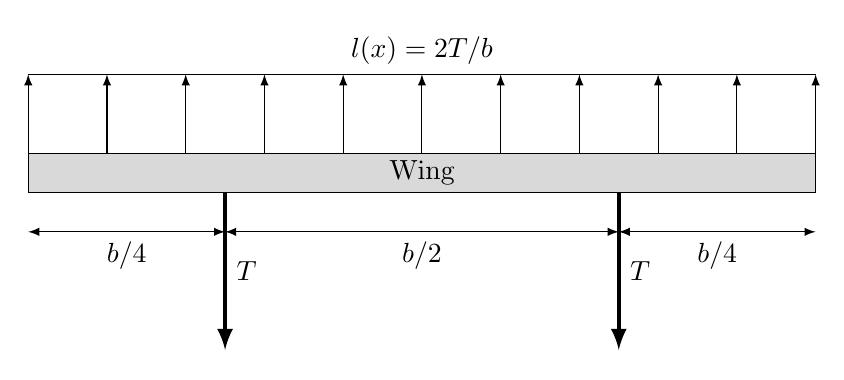
\begin{tikzpicture}
        % Wing rectangle
        \draw[fill=gray!30] (0.0, 0.0) rectangle (10.0, 0.5)
        node[pos=0.5] {Wing};

        % Distributed lift force.
        \draw (0.0, 1.5) -- (10.0, 1.5) node[midway, above] {$l(x) = 2T/b$};
        \foreach \x in {0.0, 1.0, ..., 10.0} {
          \draw[-latex] (\x, 0.5) -- (\x, 1.5);
        }

        % Bridles point loads.
        \draw[ultra thick, -latex] (2.5, 0.0) -- (2.5, -2.0)
        node[midway, right] {$T$};
        \draw[ultra thick, -latex] (7.5, 0.0) -- (7.5, -2.0)
        node[midway, right] {$T$};

        % Dimensions.
        \draw[latex-latex] (0.0, -0.5) -- (2.5, -0.5)
        node[midway, below] {$b/4$};
        \draw[latex-latex] (2.5, -0.5) -- (7.5, -0.5)
        node[midway, below] {$b/2$};
        \draw[latex-latex] (7.5, -0.5) -- (10.0, -0.5)
        node[midway, below] {$b/4$};
      \end{tikzpicture}
    \end{figure}


  \item[Problem 2] A kite is flying perpendicular to the wind with
    velocity $\vec{v}_{\mathrm{kite}}$.  The wind velocity is
    $\vec{v}_{\mathrm{wind}}$.  A tether, represented by the force
    vector $\vec{T}$, keeps the kite from flying away downwind.  The
    kite has fixed lift and drag coefficients $C_L$ and $C_D$.
    Calculate $\vec{v}_{\mathrm{kite}}$ in terms of
    $\vec{v}_{\mathrm{wind}}$, $C_L$, and $C_D$.

    \begin{figure}[h]
      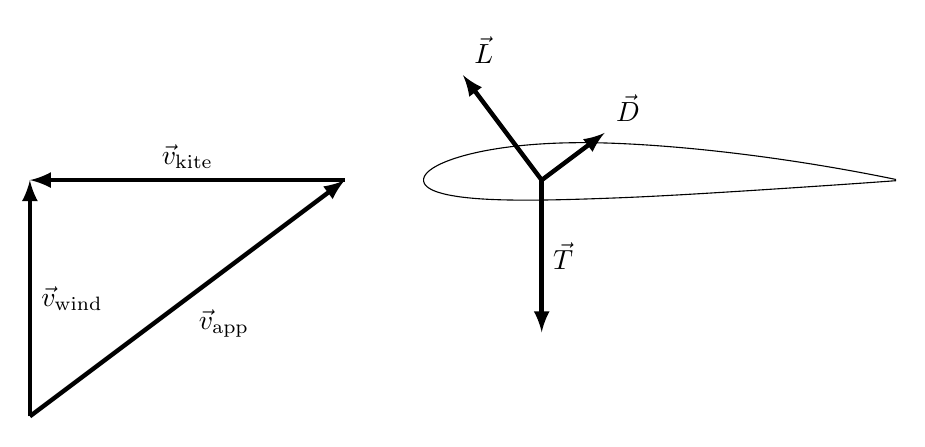
\begin{tikzpicture}
        \DrawAirfoil {6}
        % Draw velocity vectors.
        \draw[ultra thick, -latex] (-1, 0) -- (-5, 0)
        node[midway, above] {$\vec{v}_{\mathrm{kite}}$};
        \draw[ultra thick, -latex] (-5, -3) -- (-5, 0)
        node[midway, right] {$\vec{v}_{\mathrm{wind}}$};
        \draw[ultra thick, -latex] (-5, -3) -- (-1, 0)
        node[midway, below right] {$\vec{v}_{\mathrm{app}}$};

        % Draw lift, drag, tension vectors.
        \draw[ultra thick, -latex] (6/4, 0) -- ++(4/5, 3/5)
        node[above right] {$\vec{D}$};
        \draw[ultra thick, -latex] (6/4, 0) -- ++(-1, 4/3)
        node[above right] {$\vec{L}$};
        \draw[ultra thick, -latex] (6/4, 0) -- ++(0, -3/5 - 4/3)
        node[midway, right] {$\vec{T}$};
      \end{tikzpicture}
    \end{figure}

\end{description}

\end{document}
